\chapter{Modeling distributions}
\label{modeling}

The distributions we have used so far are called {\bf empirical
  distributions} because they are based on empirical observations,
which are necessarily finite samples.
\index{analytic distribution}
\index{distribution!analytic}
\index{empirical distribution}
\index{distribution!empirical}

The alternative is an {\bf analytic distribution}, which is
characterized by a CDF that is a mathematical function.
Analytic distributions can be used to model empirical distributions.
In this context, a {\bf model} is a simplification that leaves out
unneeded details.  This chapter presents common analytic distributions
and uses them to model data from a variety of sources.
\index{model}

The code for this chapter is in {\tt analytic.py}.  For information
about downloading and working with this code, see Section~\ref{code}.



\section{The exponential distribution}
\label{exponential}
\index{exponential distribution}
\index{distribution!exponential}

\begin{figure}
% analytic.py
%\centerline{\includegraphics[height=2.5in]{figs/analytic_expo_cdf.pdf}}
\caption{CDFs of exponential distributions with various parameters.}
\label{analytic_expo_cdf}
\end{figure}

I'll start with the {\bf exponential distribution} because it is
relatively simple.  The CDF of the exponential distribution is
%
\[ \CDF(x) = 1 - e^{-\lambda x} \]
%
The parameter, $\lambda$, determines the shape of the distribution.
Figure~\ref{analytic_expo_cdf} shows what this CDF looks like with
$\lambda = $ 0.5, 1, and 2.
  \index{parameter}

In the real world, exponential distributions
come up when we look at a series of events and measure the
times between events, called {\bf interarrival times}.
If the events are equally likely to occur at any time, the distribution
of interarrival times tends to look like an exponential distribution.
\index{interarrival time}

As an example, we will look at the interarrival time of births.
On December 18, 1997, 44 babies were born in a hospital in Brisbane,
Australia.\footnote{This example is based on information and data from
  Dunn, ``A Simple Dataset for Demonstrating Common Distributions,''
  Journal of Statistics Education v.7, n.3 (1999).}  The time of
birth for all 44 babies was reported in the local paper; the
complete dataset is in a file called {\tt babyboom.dat}, in the
{\tt ThinkStats2} repository.
\index{birth time}
\index{Australia} \index{Brisbane}

\begin{verbatim}
    df = ReadBabyBoom()
    diffs = df.minutes.diff()
    cdf = thinkstats2.Cdf(diffs, label='actual')

    thinkplot.Cdf(cdf)
    thinkplot.Show(xlabel='minutes', ylabel='CDF')
\end{verbatim}

{\tt ReadBabyBoom} reads the data file and returns a DataFrame
with columns {\tt time}, {\tt sex}, \verb"weight_g", and {\tt minutes},
where {\tt minutes} is time of birth converted to minutes since
midnight.
\index{DataFrame}
\index{thinkplot}

\begin{figure}
% analytic.py
%\centerline{\includegraphics[height=2.5in]{figs/analytic_interarrivals.pdf}}
\caption{CDF of interarrival times (left) and CCDF on a log-y scale (right).}
\label{analytic_interarrival_cdf}
\end{figure}

%\begin{figure}
% analytic.py
%%\centerline{\includegraphics[height=2.5in]{figs/analytic_interarrivals_logy.pdf}}
%\caption{CCDF of interarrival times.}
%\label{analytic_interarrival_ccdf}
%\end{figure}

{\tt diffs} is the difference between consecutive birth times, and
{\tt cdf} is the distribution of these interarrival times.
Figure~\ref{analytic_interarrival_cdf} (left) shows the CDF.  It seems
to have the general shape of an exponential distribution, but how can
we tell?

One way is to plot the {\bf complementary CDF}, which is $1 - \CDF(x)$,
on a log-y scale.  For data from an exponential distribution, the
result is a straight line.  Let's see why that works.
\index{complementary CDF} \index{CDF!complementary} \index{CCDF}

If you plot the complementary CDF (CCDF) of a dataset that you think is
exponential, you expect to see a function like:
%
\[ y \approx e^{-\lambda x} \]
%
Taking the log of both sides yields:
%
\[ \log y \approx -\lambda x\]
%
So on a log-y scale the CCDF is a straight line
with slope $-\lambda$.  Here's how we can generate a plot like that:
\index{logarithmic scale}
\index{complementary CDF}
\index{CDF!complementary}
\index{CCDF}


\begin{verbatim}
    thinkplot.Cdf(cdf, complement=True)
    thinkplot.Show(xlabel='minutes',
                   ylabel='CCDF',
                   yscale='log')
\end{verbatim}

With the argument {\tt complement=True}, {\tt thinkplot.Cdf} computes
the complementary CDF before plotting.  And with {\tt yscale='log'},
{\tt thinkplot.Show} sets the {\tt y} axis to a logarithmic scale.
\index{thinkplot}
\index{Cdf}

Figure~\ref{analytic_interarrival_cdf} (right) shows the result.  It is not
exactly straight, which indicates that the exponential distribution is
not a perfect model for this data.  Most likely the underlying
assumption---that a birth is equally likely at any time of day---is
not exactly true.  Nevertheless, it might be reasonable to model this
dataset with an exponential distribution.  With that simplification, we can
summarize the distribution with a single parameter.
\index{model}

The parameter, $\lambda$, can be interpreted as a rate; that is, the
number of events that occur, on average, in a unit of time.  In this
example, 44 babies are born in 24 hours, so the rate is $\lambda =
0.0306$ births per minute.  The mean of an exponential distribution is
$1/\lambda$, so the mean time between births is 32.7 minutes.


\section{The normal distribution}
\label{normal}

The {\bf normal distribution}, also called Gaussian, is commonly
used because it describes many phenomena, at least approximately.
It turns out that there is a good reason for its ubiquity, which we
will get to in Section~\ref{CLT}.
\index{CDF}
\index{parameter}
\index{mean}
\index{standard deviation}
\index{normal distribution}
\index{distribution!normal}
\index{Gaussian distribution}
\index{distribution!Gaussian}

%
%\[ \CDF(z) = \frac{1}{\sqrt{2 \pi}} \int_{-\infty}^z e^{-t^2/2} dt \]
%

\begin{figure}
% analytic.py
%\centerline{\includegraphics[height=2.5in]{figs/analytic_gaussian_cdf.pdf}}
\caption{CDF of normal distributions with a range of parameters.}
\label{analytic_gaussian_cdf}
\end{figure}

The normal distribution is characterized by two parameters: the mean,
$\mu$, and standard deviation $\sigma$.  The normal distribution with
$\mu=0$ and $\sigma=1$ is called the {\bf standard normal
  distribution}.  Its CDF is defined by an integral that does not have
a closed form solution, but there are algorithms that evaluate it
efficiently.  One of them is provided by SciPy: {\tt scipy.stats.norm}
is an object that represents a normal distribution; it provides a
method, {\tt cdf}, that evaluates the standard normal CDF:
\index{SciPy}
\index{closed form}

\begin{verbatim}
>>> import scipy.stats
>>> scipy.stats.norm.cdf(0)
0.5
\end{verbatim}

This result is correct: the median of the standard normal distribution
is 0 (the same as the mean), and half of the values fall below the
median, so $\CDF(0)$ is 0.5.

{\tt norm.cdf} takes optional parameters: {\tt loc}, which
specifies the mean, and {\tt scale}, which specifies the
standard deviation.

{\tt thinkstats2} makes this function a little easier to use
by providing {\tt EvalNormalCdf}, which takes parameters {\tt mu}
and {\tt sigma} and evaluates the CDF at {\tt x}:
\index{normal distribution}

\begin{verbatim}
def EvalNormalCdf(x, mu=0, sigma=1):
    return scipy.stats.norm.cdf(x, loc=mu, scale=sigma)
\end{verbatim}

Figure~\ref{analytic_gaussian_cdf} shows CDFs for normal
distributions with a range of parameters.  The sigmoid shape of these
curves is a recognizable characteristic of a normal distribution.

In the previous chapter we looked at the distribution of birth
weights in the NSFG.  Figure~\ref{analytic_birthwgt_model} shows the
empirical CDF of weights for all live births and the CDF of
a normal distribution with the same mean and variance.
\index{National Survey of Family Growth}
\index{NSFG}
\index{birth weight}
\index{weight!birth}

\begin{figure}
% analytic.py
%\centerline{\includegraphics[height=2.5in]{figs/analytic_birthwgt_model.pdf}}
\caption{CDF of birth weights with a normal model.}
\label{analytic_birthwgt_model}
\end{figure}

The normal distribution is a good model for this dataset, so
if we summarize the distribution with the parameters
$\mu = 7.28$ and $\sigma = 1.24$, the resulting error
(difference between the model and the data) is small.
\index{model}
\index{percentile}

Below the 10th percentile there is a discrepancy between the data
and the model; there are more light babies than we would expect in
a normal distribution.  If we are specifically interested in preterm
babies, it would be important to get this part of the distribution
right, so it might not be appropriate to use the normal
model.


\section{Normal probability plot}

For the exponential distribution, and a few others, there are
simple transformations we can use to test whether an analytic
distribution is a good model for a dataset.
\index{exponential distribution}
\index{distribution!exponential}
\index{model}

For the normal distribution there is no such transformation, but there
is an alternative called a {\bf normal probability plot}.  There
are two ways to generate a normal probability plot: the hard way
and the easy way.  If you are interested in the hard way, you can
read about it at \url{https://en.wikipedia.org/wiki/Normal_probability_plot}.
Here's the easy way:
\index{normal probability plot}
\index{plot!normal probability}
\index{normal distribution}
\index{distribution!normal}
\index{Gaussian distribution}
\index{distribution!Gaussian}

\begin{enumerate}

\item Sort the values in the sample.

\item From a standard normal distribution ($\mu=0$ and $\sigma=1$),
generate a random sample with the same size as the sample, and sort it.
\index{random number}

\item Plot the sorted values from the sample versus the random values.

\end{enumerate}

If the distribution of the sample is approximately normal, the result
is a straight line with intercept {\tt mu} and slope {\tt sigma}.
{\tt thinkstats2} provides {\tt NormalProbability}, which takes a
sample and returns two NumPy arrays:
\index{NumPy}

\begin{verbatim}
xs, ys = thinkstats2.NormalProbability(sample)
\end{verbatim}

\begin{figure}
% analytic.py
%\centerline{\includegraphics[height=2.5in]{figs/analytic_normal_prob_example.pdf}}
\caption{Normal probability plot for random samples from normal distributions.}
\label{analytic_normal_prob_example}
\end{figure}

{\tt ys} contains the sorted values from {\tt sample}; {\tt xs}
contains the random values from the standard normal distribution.

To test {\tt NormalProbability} I generated some fake samples that
were actually drawn from normal distributions with various parameters.
Figure~\ref{analytic_normal_prob_example} shows the results.
The lines are approximately straight, with values in the tails
deviating more than values near the mean.

Now let's try it with real data.  Here's code to generate
a normal probability plot for the birth weight data from the
previous section.  It plots a gray line that represents the model
and a blue line that represents the data.
\index{birth weight}
\index{weight!birth}

\begin{verbatim}
def MakeNormalPlot(weights):
    mean = weights.mean()
    std = weights.std()

    xs = [-4, 4]
    fxs, fys = thinkstats2.FitLine(xs, inter=mean, slope=std)
    thinkplot.Plot(fxs, fys, color='gray', label='model')

    xs, ys = thinkstats2.NormalProbability(weights)
    thinkplot.Plot(xs, ys, label='birth weights')
\end{verbatim}

{\tt weights} is a pandas Series of birth weights;
{\tt mean} and {\tt std} are the mean and standard deviation.
\index{pandas}
\index{Series}
\index{thinkplot}
\index{standard deviation}

{\tt FitLine} takes a sequence of {\tt xs}, an intercept, and a
slope; it returns {\tt xs} and {\tt ys} that represent a line
with the given parameters, evaluated at the values in {\tt xs}.

{\tt NormalProbability} returns {\tt xs} and {\tt ys} that
contain values from the standard normal distribution and values
from {\tt weights}.  If the distribution of weights is normal,
the data should match the model.
\index{model}

\begin{figure}
% analytic.py
%\centerline{\includegraphics[height=2.5in]{figs/analytic_birthwgt_normal.pdf}}
\caption{Normal probability plot of birth weights.}
\label{analytic_birthwgt_normal}
\end{figure}

Figure~\ref{analytic_birthwgt_normal} shows the results for
all live births, and also for full term births (pregnancy length greater
than 36 weeks).  Both curves match the model near the mean and
deviate in the tails.  The heaviest babies are heavier than what
the model expects, and the lightest babies are lighter.
\index{pregnancy length}

When we select only full term births, we remove some of the lightest
weights, which reduces the discrepancy in the lower tail of the
distribution.

This plot suggests that the normal model describes the distribution
well within a few standard deviations from the mean, but not in the
tails.  Whether it is good enough for practical purposes depends
on the purposes.
\index{model}
\index{birth weight}
\index{weight!birth}
\index{standard deviation}


\section{The lognormal distribution}
\label{brfss}
\label{lognormal}

If the logarithms of a set of values have a normal distribution, the
values have a {\bf lognormal distribution}.  The CDF of the lognormal
distribution is the same as the CDF of the normal distribution,
with $\log x$ substituted for $x$.
%
\[ CDF_{lognormal}(x) = CDF_{normal}(\log x)\]
%
The parameters of the lognormal distribution are usually denoted
$\mu$ and $\sigma$.  But remember that these parameters are {\em not}
the mean and standard deviation; the mean of a lognormal distribution
is $\exp(\mu +\sigma^2/2)$ and the standard deviation is
ugly (see \url{http://wikipedia.org/wiki/Log-normal_distribution}).
\index{parameter} \index{weight!adult} \index{adult weight}
\index{lognormal distribution}
\index{distribution!lognormal}
\index{CDF}

\begin{figure}
% brfss.py
%\centerline{
%\includegraphics[height=2.5in]{figs/brfss_weight.pdf}}
%\caption{CDF of adult weights on a linear scale (left) and
%log scale (right).}
%\label{brfss_weight}
\end{figure}

If a sample is approximately lognormal and you plot its CDF on a
log-x scale, it will have the characteristic shape of a normal
distribution.  To test how well the sample fits a lognormal model, you
can make a normal probability plot using the log of the values
in the sample.
\index{normal probability plot}
\index{model}

As an example, let's look at the distribution of adult weights, which
is approximately lognormal.\footnote{I was tipped off to this
  possibility by a comment (without citation) at
  \url{http://mathworld.wolfram.com/LogNormalDistribution.html}.
  Subsequently I found a paper that proposes the log transform and
  suggests a cause: Penman and Johnson, ``The Changing Shape of the
  Body Mass Index Distribution Curve in the Population,'' Preventing
  Chronic Disease, 2006 July; 3(3): A74.  Online at
  \url{http://www.ncbi.nlm.nih.gov/pmc/articles/PMC1636707}.}

The National Center for Chronic Disease
Prevention and Health Promotion conducts an annual survey as part of
the Behavioral Risk Factor Surveillance System
(BRFSS).\footnote{Centers for Disease Control and Prevention
  (CDC). Behavioral Risk Factor Surveillance System Survey
  Data. Atlanta, Georgia: U.S. Department of Health and Human
  Services, Centers for Disease Control and Prevention, 2008.}  In
2008, they interviewed 414,509 respondents and asked about their
demographics, health, and health risks.
Among the data they collected are the weights in kilograms of
398,484 respondents.
\index{Behavioral Risk Factor Surveillance System}
\index{BRFSS}

The repository for this book contains {\tt CDBRFS08.ASC.gz},
a fixed-width ASCII file that contains data from the BRFSS,
and {\tt brfss.py}, which reads the file and analyzes the data.

\begin{figure}
% brfss.py
%\centerline{
%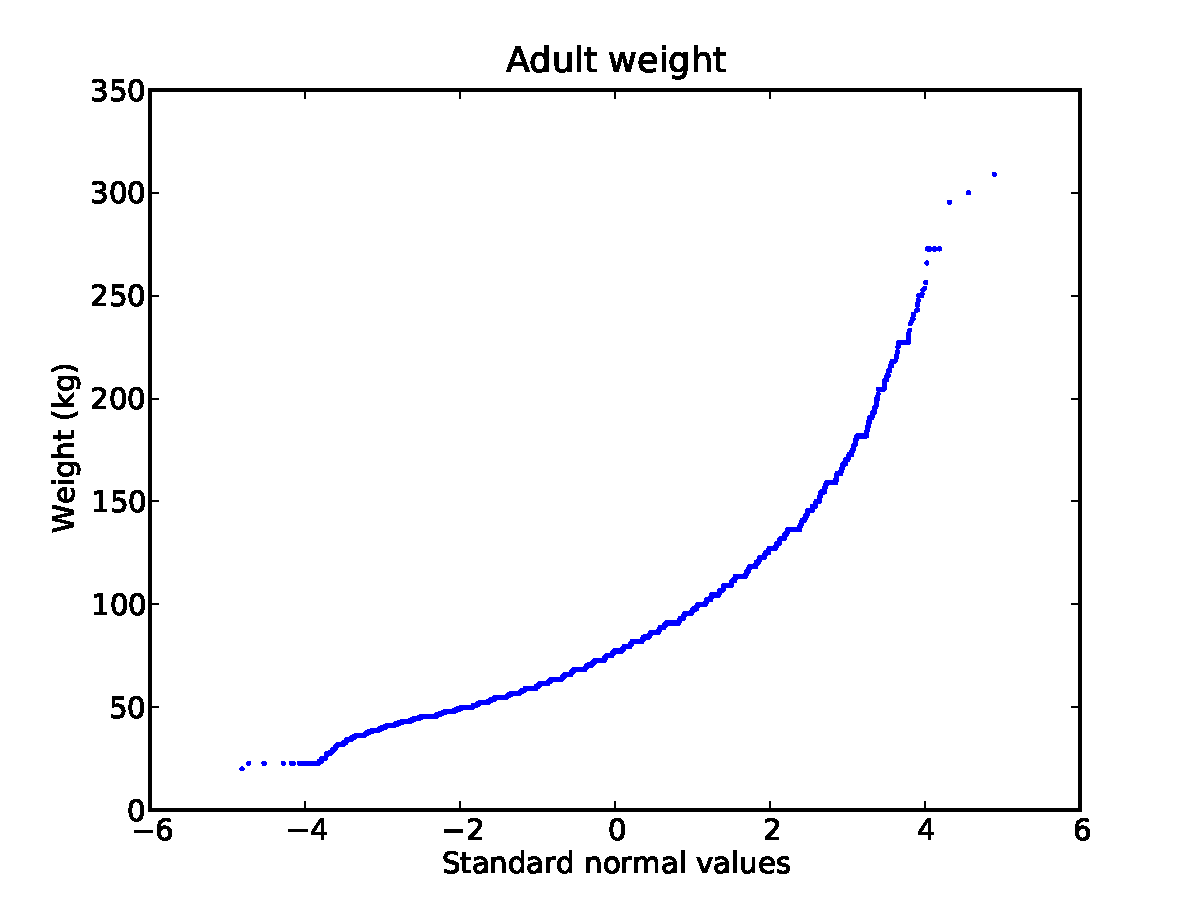
\includegraphics[height=2.5in]{figs/brfss_weight_normal.pdf}}
\caption{Normal probability plots for adult weight on a linear scale
  (left) and log scale (right).}
\label{brfss_weight_normal}
\end{figure}

Figure~\ref{brfss_weight} (left) shows the distribution of adult
weights on a linear scale with a normal model.
Figure~\ref{brfss_weight} (right) shows the same distribution on a log
scale with a lognormal model.  The lognormal model is a better fit,
but this representation of the data does not make the difference
particularly dramatic.  \index{respondent} \index{model}

Figure~\ref{brfss_weight_normal} shows normal probability plots for
adult weights, $w$, and for their logarithms, $\log_{10} w$.  Now it
is apparent that the data deviate substantially from the normal model.
On the other hand, the lognormal model is a good match for the data.
\index{normal distribution} \index{distribution!normal}
\index{Gaussian distribution} \index{distribution!Gaussian}
\index{lognormal distribution} \index{distribution!lognormal}
\index{standard deviation} \index{adult weight} \index{weight!adult}
\index{model} \index{normal probability plot}


\section{The Pareto distribution}
\index{Pareto distribution}
\index{distribution!Pareto}
\index{Pareto, Vilfredo}

The {\bf Pareto distribution} is named after the economist Vilfredo Pareto,
who used it to describe the distribution of wealth (see
\url{http://wikipedia.org/wiki/Pareto_distribution}).  Since then, it
has been used to describe phenomena in the natural and social sciences
including sizes of cities and towns, sand particles and meteorites,
forest fires and earthquakes.  \index{CDF}

The CDF of the Pareto distribution is:
%
\[ CDF(x) = 1 - \left( \frac{x}{x_m} \right) ^{-\alpha} \]
%
The parameters $x_{m}$ and $\alpha$ determine the location and shape
of the distribution. $x_{m}$ is the minimum possible value.
Figure~\ref{analytic_pareto_cdf} shows CDFs of Pareto
distributions with $x_{m} = 0.5$ and different values
of $\alpha$.
\index{parameter}

\begin{figure}
% analytic.py
%\centerline{\includegraphics[height=2.5in]{figs/analytic_pareto_cdf.pdf}}
\caption{CDFs of Pareto distributions with different parameters.}
\label{analytic_pareto_cdf}
\end{figure}

There is a simple visual test that indicates whether an empirical
distribution fits a Pareto distribution: on a log-log scale, the CCDF
looks like a straight line.  Let's see why that works.

If you plot the CCDF of a sample from a Pareto distribution on a
linear scale, you expect to see a function like:
%
\[ y \approx \left( \frac{x}{x_m} \right) ^{-\alpha} \]
%
Taking the log of both sides yields:
%
\[ \log y \approx -\alpha (\log x - \log x_{m})\]
%
So if you plot $\log y$ versus $\log x$, it should look like a straight
line with slope $-\alpha$ and intercept
$\alpha \log x_{m}$.

As an example, let's look at the sizes of cities and towns.
The U.S.~Census Bureau publishes the
population of every incorporated city and town in the United States.
\index{Pareto distribution} \index{distribution!Pareto}
\index{U.S.~Census Bureau} \index{population} \index{city size}

\begin{figure}
% populations.py
%\centerline{\includegraphics[height=2.5in]{figs/populations_pareto.pdf}}
\caption{CCDFs of city and town populations, on a log-log scale.}
\label{populations_pareto}
\end{figure}

I downloaded their data from
\url{http://www.census.gov/popest/data/cities/totals/2012/SUB-EST2012-3.html};
it is in the repository for this book in a file named
\verb"PEP_2012_PEPANNRES_with_ann.csv".  The repository also
contains {\tt populations.py}, which reads the file and plots
the distribution of populations.

Figure~\ref{populations_pareto} shows the CCDF of populations on a
log-log scale.  The largest 1\% of cities and towns, below $10^{-2}$,
fall along a straight line.  So we could
conclude, as some researchers have, that the tail of this distribution
fits a Pareto model.
\index{model}

On the other hand, a lognormal distribution also models the data well.
Figure~\ref{populations_normal} shows the CDF of populations and a
lognormal model (left), and a normal probability plot (right).  Both
plots show good agreement between the data and the model.
\index{normal probability plot}

Neither model is perfect.
The Pareto model only applies to the largest 1\% of cities, but it
is a better fit for that part of the distribution.  The lognormal
model is a better fit for the other 99\%.
Which model is appropriate depends on which part of the distribution
is relevant.

\begin{figure}
% populations.py
%\centerline{\includegraphics[height=2.5in]{figs/populations_normal.pdf}}
\caption{CDF of city and town populations on a log-x scale (left), and
normal probability plot of log-transformed populations (right).}
\label{populations_normal}
\end{figure}


\section{Generating random numbers}
\index{exponential distribution}
\index{distribution!exponential}
\index{random number}
\index{CDF}
\index{inverse CDF algorithm}
\index{uniform distribution}
\index{distribution!uniform}

Analytic CDFs can be used to generate random numbers with a given
distribution function, $p = \CDF(x)$.  If there is an efficient way to
compute the inverse CDF, we can generate random values
with the appropriate distribution by choosing $p$ from a uniform
distribution between 0 and 1, then choosing
$x = ICDF(p)$.
\index{inverse CDF}
\index{CDF, inverse}

For example, the CDF of the exponential distribution is
%
\[ p = 1 - e^{-\lambda x} \]
%
Solving for $x$ yields:
%
\[ x = -\log (1 - p) / \lambda \]
%
So in Python we can write
%
\begin{verbatim}
def expovariate(lam):
    p = random.random()
    x = -math.log(1-p) / lam
    return x
\end{verbatim}

{\tt expovariate} takes {\tt lam} and returns a random value chosen
from the exponential distribution with parameter {\tt lam}.

Two notes about this implementation:
I called the parameter \verb"lam" because \verb"lambda" is a Python
keyword.  Also, since $\log 0$ is undefined, we have to
be a little careful.  The implementation of {\tt random.random}
can return 0 but not 1, so $1 - p$ can be 1 but not 0, so
{\tt log(1-p)} is always defined.  \index{random module}


\section{Why model?}
\index{model}

At the beginning of this chapter, I said that many real world phenomena
can be modeled with analytic distributions.  ``So,'' you might ask,
``what?''  \index{abstraction}

Like all models, analytic distributions are abstractions, which
means they leave out details that are considered irrelevant.
For example, an observed distribution might have measurement errors
or quirks that are specific to the sample; analytic models smooth
out these idiosyncrasies.
\index{smoothing}

Analytic models are also a form of data compression.  When a model
fits a dataset well, a small set of parameters can summarize a
large amount of data.
\index{parameter}
\index{compression}

It is sometimes surprising when data from a natural phenomenon fit an
analytic distribution, but these observations can provide insight
into physical systems.  Sometimes we can explain why an observed
distribution has a particular form.  For example, Pareto distributions
are often the result of generative processes with positive feedback
(so-called preferential attachment processes: see
\url{http://wikipedia.org/wiki/Preferential_attachment}.).
\index{preferential attachment}
\index{generative process}
\index{Pareto distribution}
\index{distribution!Pareto}
\index{analysis}

Also, analytic distributions lend themselves to mathematical
analysis, as we will see in Chapter~\ref{analysis}.

But it is important to remember that all models are imperfect.
Data from the real world never fit an analytic distribution perfectly.
People sometimes talk as if data are generated by models; for example,
they might say that the distribution of human heights is normal,
or the distribution of income is lognormal.  Taken literally, these
claims cannot be true; there are always differences between the
real world and mathematical models.

Models are useful if they capture the relevant aspects of the
real world and leave out unneeded details.  But what is ``relevant''
or ``unneeded'' depends on what you are planning to use the model
for.


\section{Exercises}

For the following exercises, you can start with \verb"chap05ex.ipynb".
My solution is in \verb"chap05soln.ipynb".

\begin{exercise}
In the BRFSS (see Section~\ref{lognormal}), the distribution of
heights is roughly normal with parameters $\mu = 178$ cm and
$\sigma = 7.7$ cm for men, and $\mu = 163$ cm and $\sigma = 7.3$ cm for
women.
\index{normal distribution}
\index{distribution!normal}
\index{Gaussian distribution}
\index{distribution!Gaussian}
\index{height}
\index{Blue Man Group}
\index{Group, Blue Man}

In order to join Blue Man Group, you have to be male between 5'10''
and 6'1'' (see \url{http://bluemancasting.com}).  What percentage of
the U.S. male population is in this range?  Hint: use {\tt
  scipy.stats.norm.cdf}.
\index{SciPy}

\end{exercise}


\begin{exercise}
To get a feel for the Pareto distribution, let's see how different
the world
would be if the distribution of human height were Pareto.
With the parameters $x_{m} = 1$ m and $\alpha = 1.7$, we
get a distribution with a reasonable minimum, 1 m,
and median, 1.5 m.
\index{height}
\index{Pareto distribution}
\index{distribution!Pareto}

Plot this distribution.  What is the mean human height in Pareto
world?  What fraction of the population is shorter than the mean?  If
there are 7 billion people in Pareto world, how many do we expect to
be taller than 1 km?  How tall do we expect the tallest person to be?
\index{Pareto World}

\end{exercise}


\begin{exercise}
\label{weibull}

The Weibull distribution is a generalization of the exponential
distribution that comes up in failure analysis
(see \url{http://wikipedia.org/wiki/Weibull_distribution}).  Its CDF is
%
\[ CDF(x) = 1 - e^{-(x / \lambda)^k} \]
%
Can you find a transformation that makes a Weibull distribution look
like a straight line?  What do the slope and intercept of the
line indicate?
\index{Weibull distribution}
\index{distribution!Weibull}
\index{exponential distribution}
\index{distribution!exponential}
\index{random module}

Use {\tt random.weibullvariate} to generate a sample from a
Weibull distribution and use it to test your transformation.

\end{exercise}


\begin{exercise}
For small values of $n$, we don't expect an empirical distribution
to fit an analytic distribution exactly.  One way to evaluate
the quality of fit is to generate a sample from an analytic
distribution and see how well it matches the data.
\index{empirical distribution}
\index{distribution!empirical}
\index{random module}

For example, in Section~\ref{exponential} we plotted the distribution
of time between births and saw that it is approximately exponential.
But the distribution is based on only 44 data points.  To see whether
the data might have come from an exponential distribution, generate 44
values from an exponential distribution with the same mean as the
data, about 33 minutes between births.

Plot the distribution of the random values and compare it to the
actual distribution.  You can use {\tt random.expovariate} 
to generate the values.

\end{exercise}

\begin{exercise}
In the repository for this book, you'll find a set of data files
called {\tt mystery0.dat}, {\tt mystery1.dat}, and so on.  Each
contains a sequence of random numbers generated from an analytic
distribution.
\index{random number}

You will also find \verb"test_models.py", a script that reads
data from a file and plots the CDF under a variety of transforms.
You can run it like this:

\begin{verbatim}
$ python test_models.py mystery0.dat
\end{verbatim}

Based on these plots, you should be able to infer what kind of
distribution generated each file.  If you are stumped, you can
look in {\tt mystery.py}, which contains the code that generated
the files.

\end{exercise}


\begin{exercise}
\label{income}

The distributions of wealth and income are sometimes modeled using
lognormal and Pareto distributions.  To see which is better, let's
look at some data.
\index{Pareto distribution}
\index{distribution!Pareto}
\index{lognormal distribution}
\index{distribution!lognormal}

The Current Population Survey (CPS) is a joint effort of the Bureau
of Labor Statistics and the Census Bureau to study income and related
variables.  Data collected in 2013 is available from
\url{http://www.census.gov/hhes/www/cpstables/032013/hhinc/toc.htm}.
I downloaded {\tt hinc06.xls}, which is an Excel spreadsheet with
information about household income, and converted it to {\tt hinc06.csv},
a CSV file you will find in the repository for this book.  You
will also find {\tt hinc.py}, which reads this file.

Extract the distribution of incomes from this dataset.  Are any of the
analytic distributions in this chapter a good model of the data?  A
solution to this exercise is in \url{hinc_soln.py}.
\index{model}

\end{exercise}




\section{Glossary}

\begin{itemize}

\item empirical distribution: The distribution of values in a sample.
  \index{empirical distribution} \index{distribution!empirical}

\item analytic distribution: A distribution whose CDF is an analytic
function.
\index{analytic distribution}
\index{distribution!analytic}

\item model: A useful simplification.  Analytic distributions are
often good models of more complex empirical distributions.
\index{model}

\item interarrival time: The elapsed time between two events.
\index{interarrival time}

\item complementary CDF: A function that maps from a value, $x$,
to the fraction of values that exceed $x$, which is $1 - \CDF(x)$.
\index{complementary CDF} \index{CDF!complementary} \index{CCDF}

\item standard normal distribution: The normal distribution with
mean 0 and standard deviation 1.
\index{standard normal distribution}

\item normal probability plot: A plot of the values in a sample versus
random values from a standard normal distribution.
\index{normal probability plot}
\index{plot!normal probability}

\end{itemize}

